 %esto es lo nuevo que agregue
\phantomsection
\section*{Anexos}
\addcontentsline{toc}{section}{Anexos}
\noindent 

\vspace{2mm}
        \begin{minipage}{0.9\textwidth}
        \centering
        \captionof{table}[{}]{ }
        \label{matrizgeneral}
         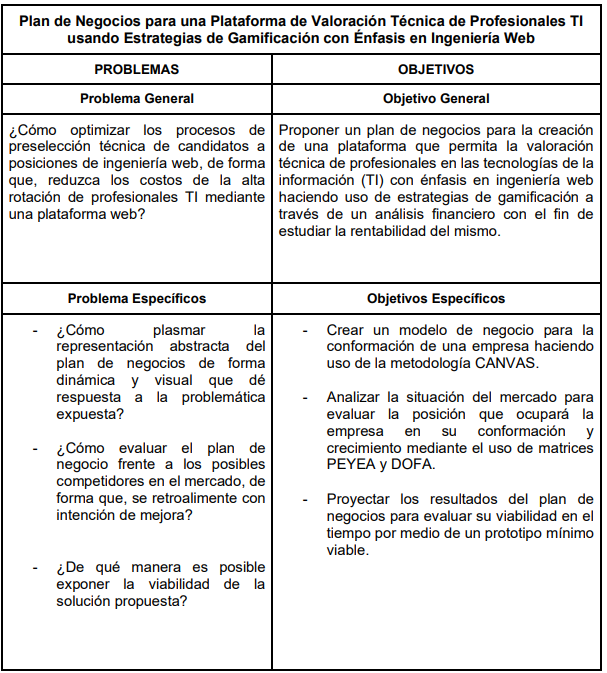
\includegraphics[width=1\textwidth]{Images/matriz general.png}
          %esto es lo nuevo que agregue
        \fnote{Nota. \textup{Fuente: Autores } }
\end{minipage}

\vspace{2mm}
        \begin{minipage}{0.9\textwidth}
        \centering
        \captionof{table}[{Matriz de los cuadros}]{Matriz de los cuadros }
        \label{cuadros}
         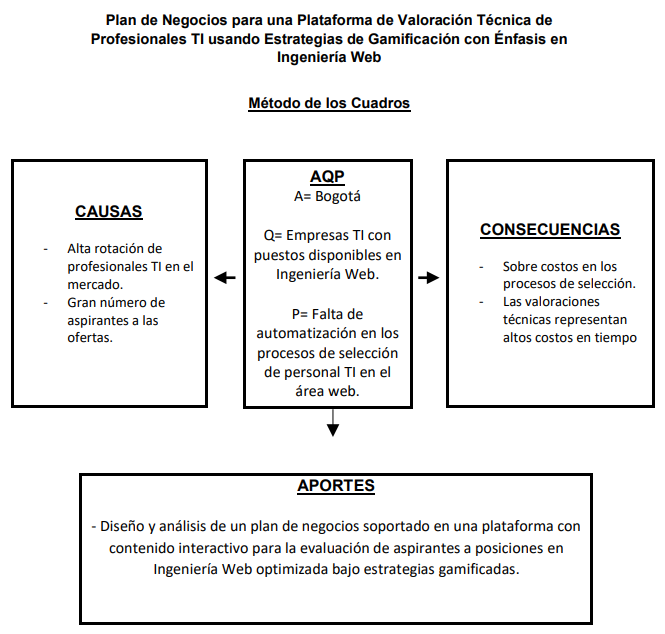
\includegraphics[width=1\textwidth]{Images/matriz de los cuadros.png}
          %esto es lo nuevo que agregue
        \fnote{Nota. \textup{Fuente: Método de los Cuadros, \cite{Rosario2020} } }
\end{minipage}

\vspace{2mm}
        \begin{minipage}{0.9\textwidth}
        \centering
        \captionof{figure}[{Aceleración de Proyectos de Emprendimiento e Innovación de la CCB-1}]{Aceleración de Proyectos de Emprendimiento e Innovación de la CCB-1 }
        \label{convocatoria1}
         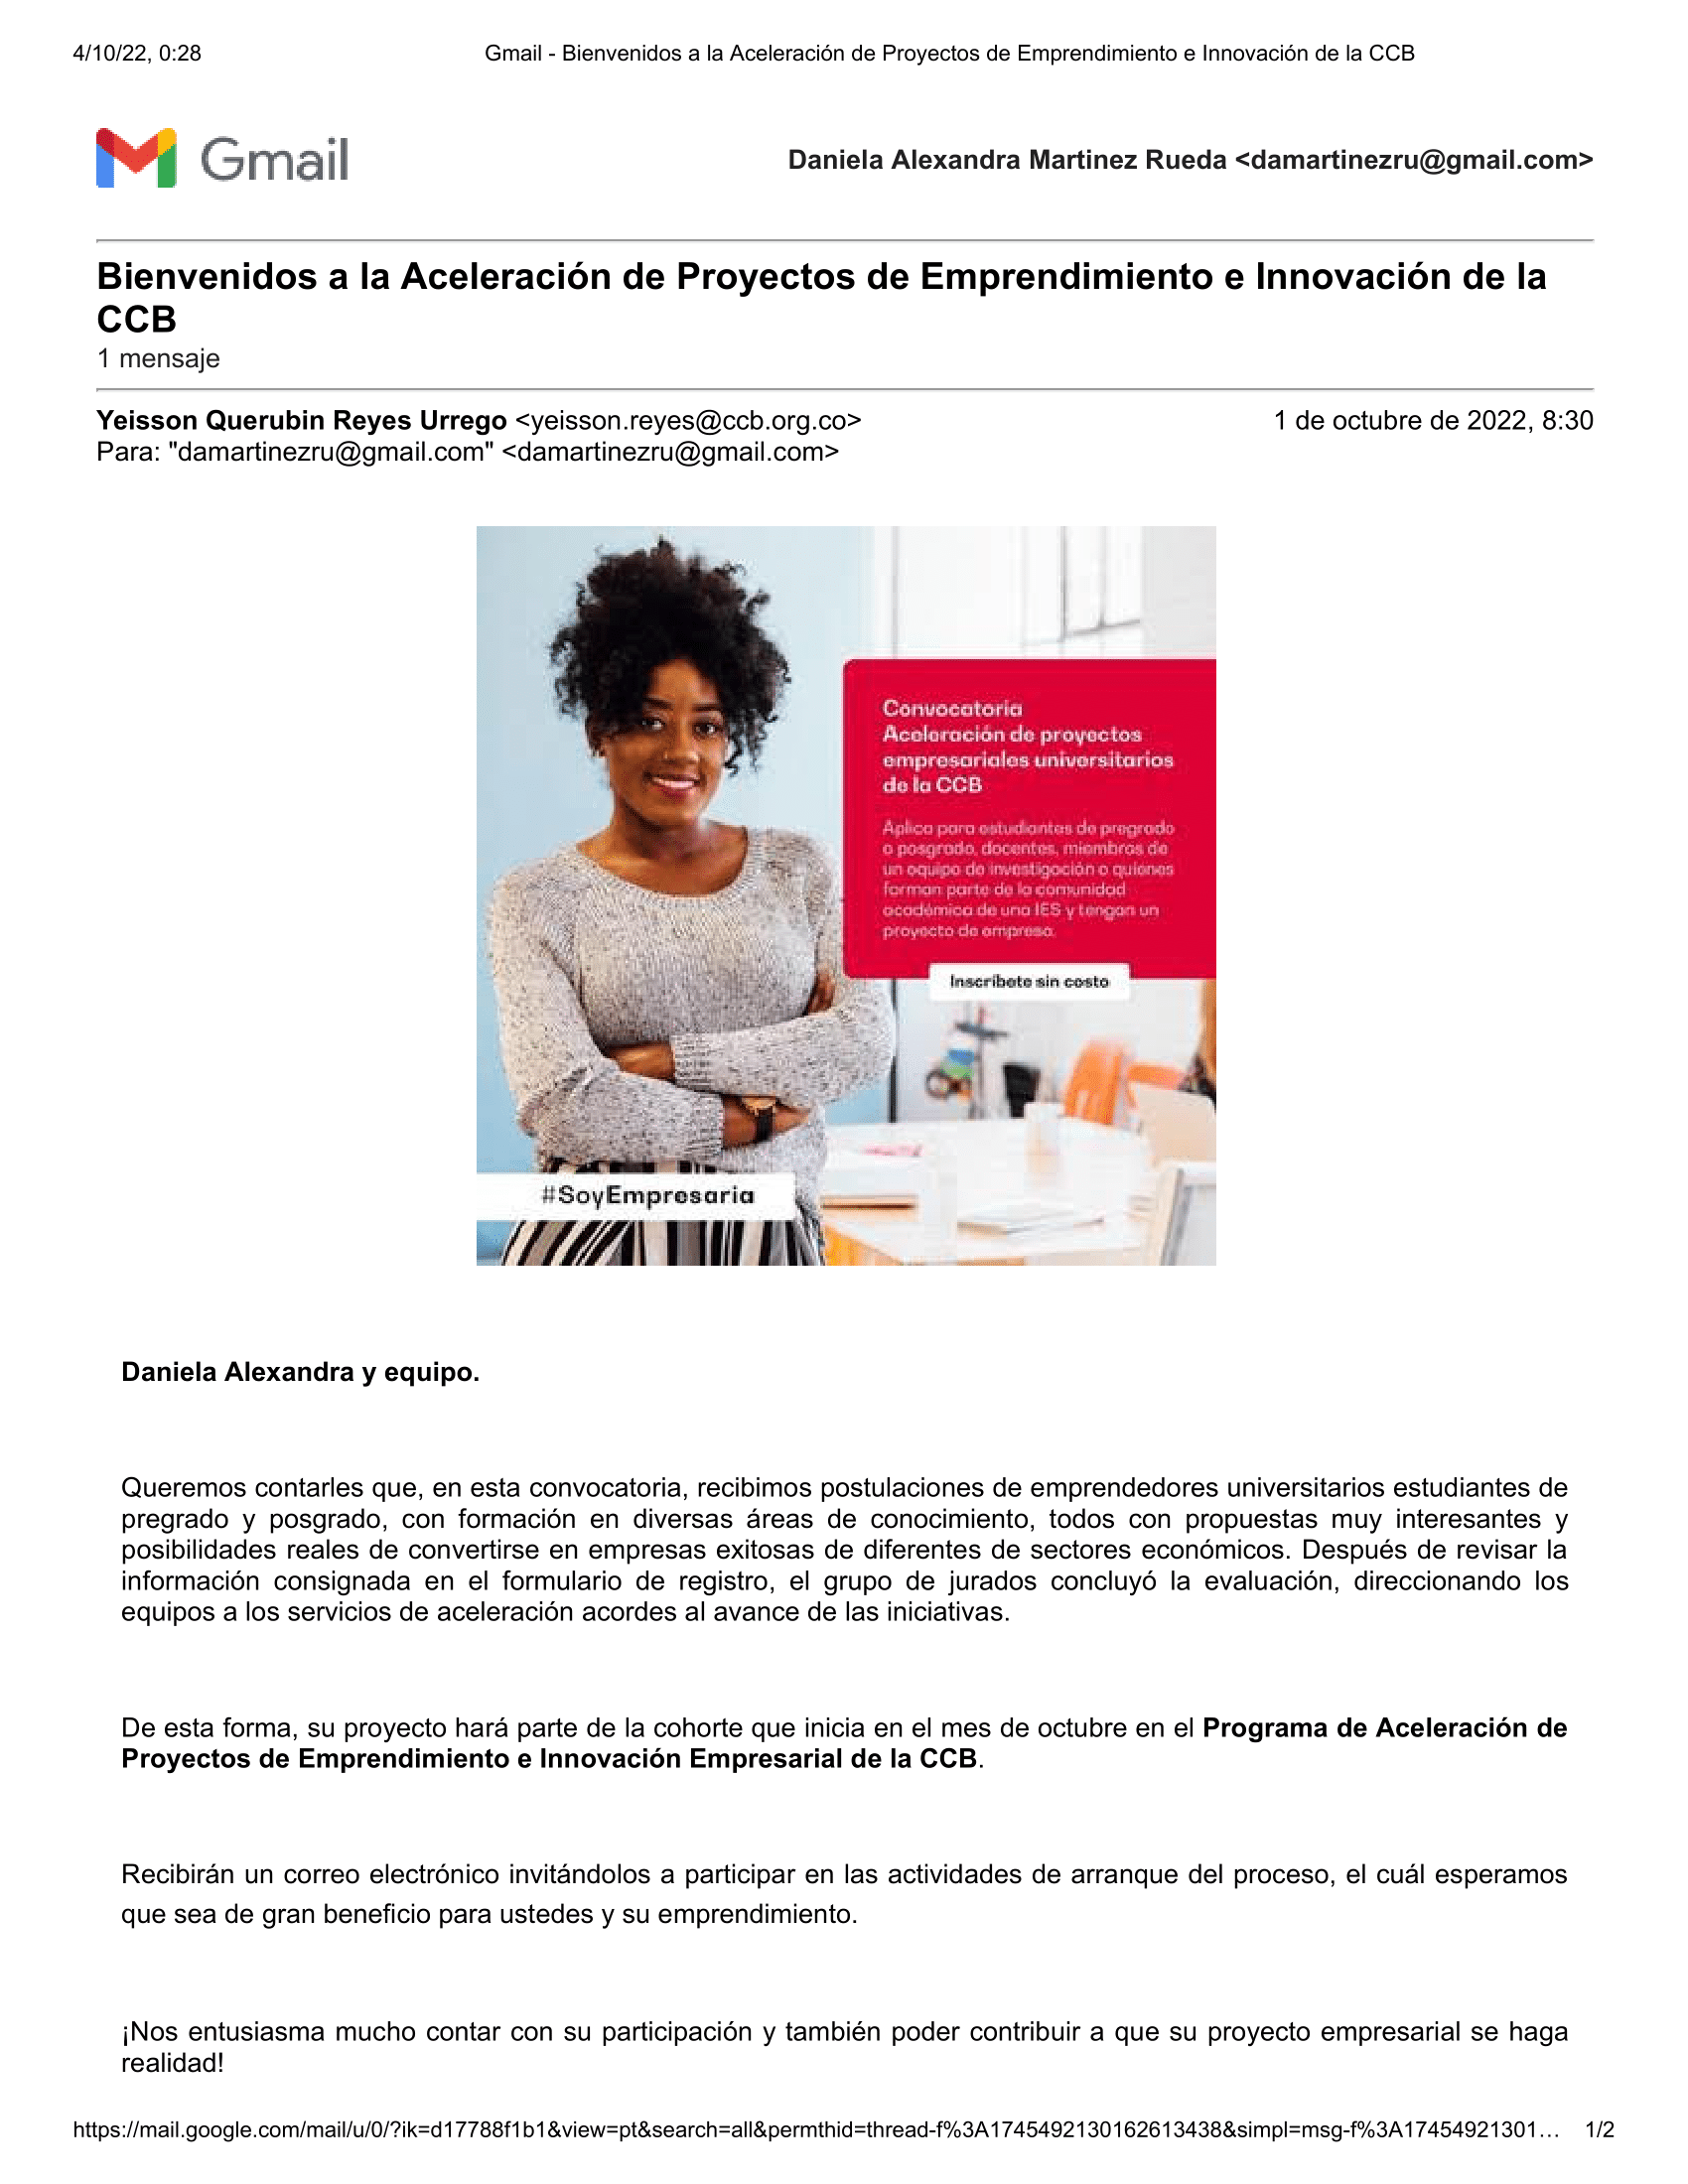
\includegraphics[width=1\textwidth]{Images/Gmail - Bienvenidos a la Aceleración de Proyectos de Emprendimiento e Innovación de la CCB-1.png}
          %esto es lo nuevo que agregue
        \fnote{Nota. \textup{Fuente: Correo Electrónico <damartinezru@gmail.com>} }
\end{minipage}

\vspace{2mm}
        \begin{minipage}{0.9\textwidth}
        \centering
        \captionof{figure}[{Aceleración de Proyectos de Emprendimiento e Innovación de la CCB-2 }]{Aceleración de Proyectos de Emprendimiento e Innovación de la CCB-2 }
        \label{convocatoria1}
         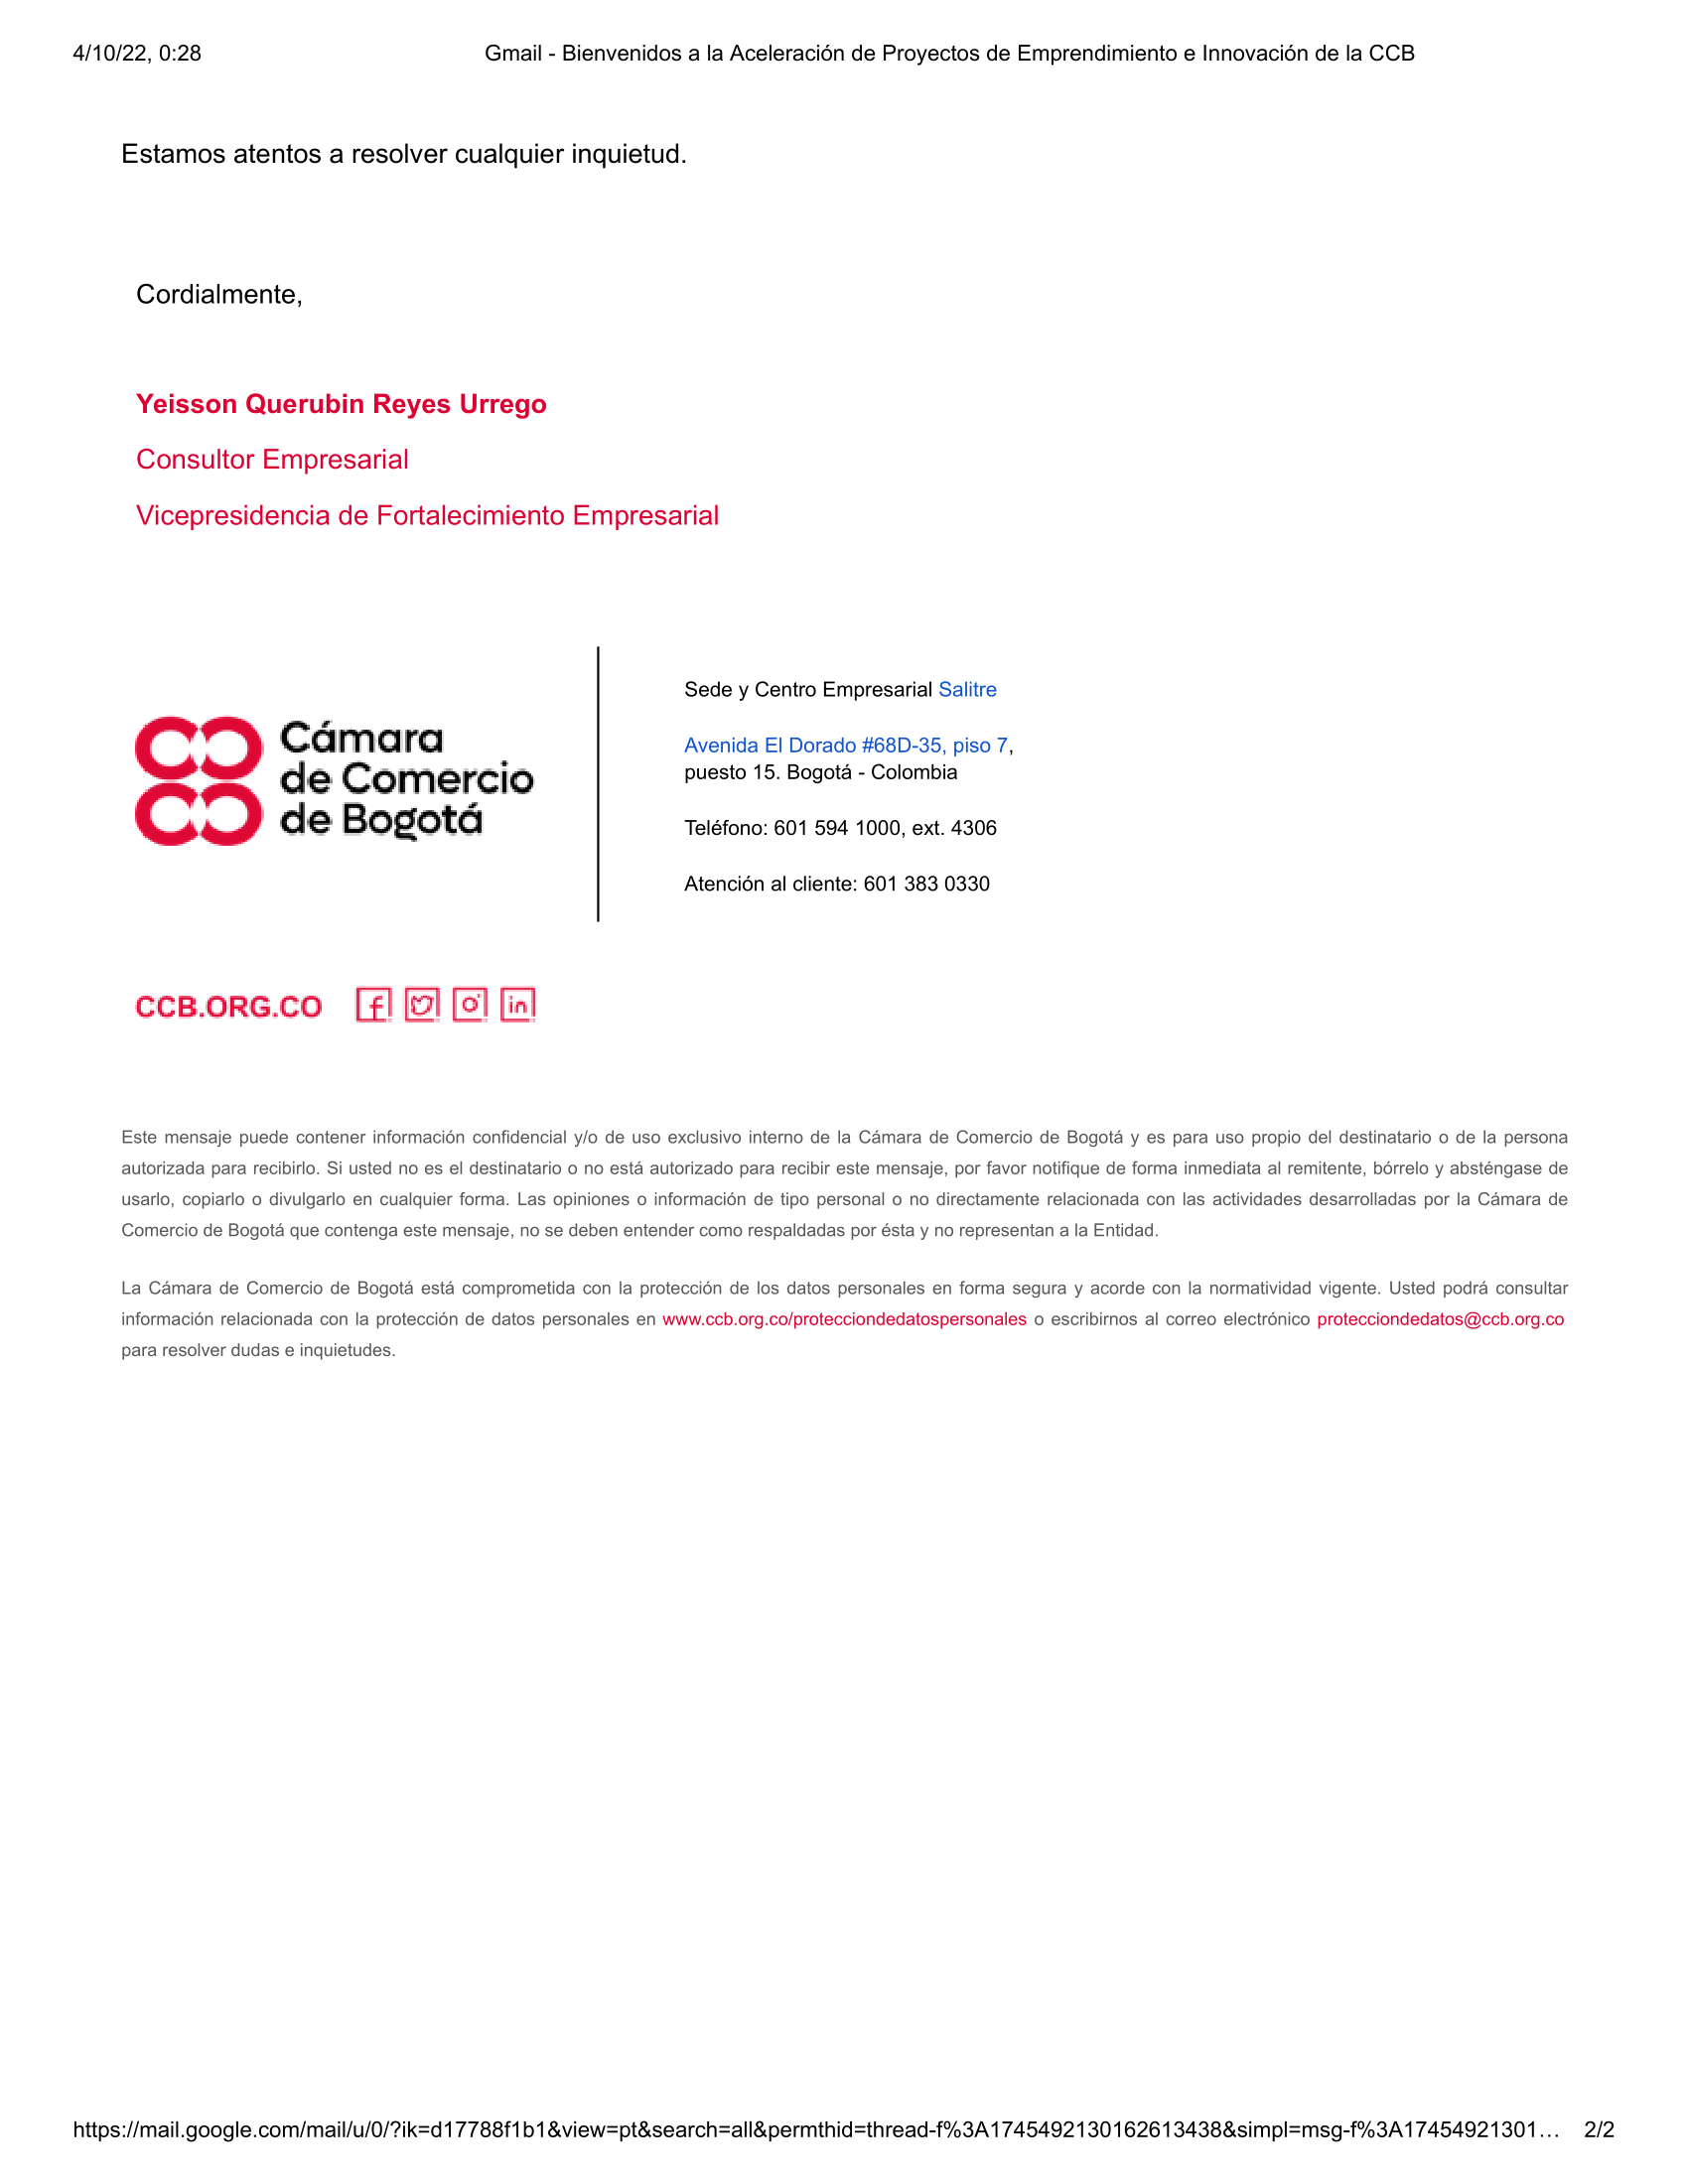
\includegraphics[width=1\textwidth]{Images/Gmail - Bienvenidos a la Aceleración de Proyectos de Emprendimiento e Innovación de la CCB-2.png}
          %esto es lo nuevo que agregue
        \fnote{Nota. \textup{Fuente: Correo Electrónico <damartinezru@gmail.com>} }
\end{minipage}